%%%%%%%%%%%%%%%%%%%%%%%%%%%%%%%%%%%%%%%%%%%%%%%%%%%%%%%%%%%%%%%%%%%%%%%%%%%%%%%
%
% witseiepaper-2005.tex
%
%                       Ken Nixon (12 October 2005)
%
%                       Sample Paper for ELEN417/455 2005
%
%%%%%%%%%%%%%%%%%%%%%%%%%%%%%%%%%%%%%%%%%%%%%%%%%%%%%%%%%%%%%%%%%%%%%%%%%%%%%%%%

\documentclass[11pt]{witseiepaper}

%
% All KJN's macros and goodies (some shameless borrowing from SPL)
\usepackage{KJN}
\usepackage[T1]{fontenc}
\usepackage{amsmath}
\usepackage{pgfgantt}
\usepackage{subcaption}
\usepackage{caption}
\usepackage{siunitx}
\usepackage{graphicx}
\graphicspath{{Images/}}
%
% PDF Info
%
\ifpdf
\pdfinfo{
/Title (Design Project)
/Author (Tristan Kuisis)
/CreationDate (D:201808300911)
/ModDate (D:200510121530)
/Subject (ELEN417/455 Paper Format, 2005)
/Keywords (Nothing)
}
\fi

%%%%%%%%%%%%%%%%%%%%%%%%%%%%%%%%%%%%%%%%%%%%%%%%%%%%%%%%%%%%%%%%%%%%%%%%%%%%%%%
\begin{document}

\title{Design Project}
\author{Tristan Kuisis
\thanks{School of Electrical \& Information Engineering, University of the
Witwatersrand, Private Bag 3, 2050, Johannesburg, South Africa}
}


%%%%%%%%%%%%%%%%%%%%%%%%%%%%%%%%%%%%%%%%%%%%%%%%%%%%%%%%%%%%%%%%%%%%%%%%%%%%%%%
%
\abstract{%The purpose of this document is to provide overview of the project undertaken from 16th of July to the 24th of August. 
Abstract Here}

\keywords{Keywords}


\maketitle
\thispagestyle{empty}\pagestyle{empty}


%%%%%%%%%%%%%%%%%%%%%%%%%%%%%%%%%%%%%%%%%%%%%%%%%%%%%%%%%%%%%%%%%%%%%%%%%%%%%%%
%




\section{INTRODUCTION} \label{sec:INTRODUCTION}

Over the last six decades, man has continuously propelled man made objects into space \cite{sputnik}. These objects have been said to exceed speed of $66 km/s$ \cite{fastestObject}, however, these extremely fast objects often leave the earths orbit and travel into outer space. Since the dawn of space exploration, many countries around the world have attemped, and in many cases, successfully deployed man made objects into the Earths upper atmosphere and into orbits around the Earth.

The organisations running these missions, in the early years, did not have sets of guidelines on how the missions should be carried out. In addition to this, there were many decades, during the Cold War era, that countries and organisations took extreme measures to make these missions a success. Many of the missions involved leaving many parts of the space craft in the Earths orbit \cite{spaceDebrisGuide}. Consequently, the number of debris orbiting the Earth grew over the years.
This was not thought to be an issue to the world at large as the belief was that space is immense and so there were no issues with using it as a dumping ground. It was not until the realisation by Kessler that the world began to worry \cite{Kessler}. This theory predicted that as the number of man made satellites (and other objects) in Earths orbit increases, so does the probability of collisions between them increase. When orbiting debris collide, the two objects can fragment (due to the excessive relative speeds with which the two objects travel at) and case multiple cascading collisions. This means that the debris orbiting the Earth would increase and result in greater difficulty for active space craft to undertake their missions.
Protecting active missions from this space debris is highly difficult as it is difficult to predict the density of objects in the specific orbit that the missions device should be in.

Guidelines were developed by NASA in the late 70's, however, this simply slowed the rate of introduction of debris and this did nothing to reduce the currently orbiting debris \cite{spaceDebrisGuide}. Recently, the United Nations General Assembly managed to get agreement between a number of countries to reduce the introduction of this debris \cite{debrisGuidelinesAgreement}.

There have been a number of methods in which to deal with this issue. The first is to protect the current missions from this debris, the first of these is to make use of a Whipple shield, this is simply an outer coating of space craft that is able to protect the craft against high velocity impacts of objects in outer space \cite{Whipple}. This shield is built to protect the craft from impacts from micrometeoroids in space.
This method falls short when the debris becomes large enough to penetrate the craft (and the Whipple shield), resulting in the destruction/damage of the craft.

A recent system is capable of removing debris from the Earths orbit, however, this is still in its early stages and has yet to prove highly effective \cite{removalSpaceDebris}.
The next method that systems currently make use of is object avoidance. This, however, is coupled with the fact that the location and trajectory of debris in orbit should be known and tracked. This forms the major task of this report.
Current solutions make use of either optical sensors which makes use of advanced telescopes in order to visually detect the debris. This system has a major drawback based on the fact that it can only be used during dawn and dusk hours \cite{OrbitalDebrisTechnicalAssessment,telescope,ZenithRanging}.
The second implementation makes use of radar techniques. This is the method which is implemented in this system.

This report begins with explaining the background to the task given, this includes an explanation of how the radar system works (in principle) it is then followed up with a description of the different ways in which the radar system can be implemented.
This is then followed up with a description of the space debris as well as a number of calculations on the characteristics of this debris.

Once the debris has been characterised, current implementations used for this application are analysed and compared.  

*** Need more here on the structure of the report.
% in the document: a-technical-assessment there is an image which breaks down all of the types of space debris


\subsection{Space Debris} \label{sec:SpaceDebris}
As discussed in section~\ref{sec:INTRODUCTION}, space debris in Earths orbit has been increasing for many decades, this is mainly due to space missions with poor regulations on the material that is allowed to stay in Earths orbit.
The majority of space debris currently is made up of man made air craft components, this includes objects such as: funcioning space craft, non-functional spacecraft, rocket bodies, exhaust products, objects created through deployment operations, and products of deteriorated space craft \cite{OrbitalDebrisTechnicalAssessment}.
Consequently, a large amount of this debris is made up of metallic materials as these materials make up the majority of the space crafts' components.
It has, in the past \cite{Spacex}, been difficult and costly to retrive the components which were used to get the space craft into orbit, this is a major contributer to the material.
This debris can occupy a number of regions within the Earths orbits and this changes its characteristics.
The current scope of the project is that it should be capable of tracking space debris that is within the Low Earth Orbit (LEO). This orbit is defined to be approximately $160 km$ to $2000 km$ altitude above the Earths mean sea level.
The second definition of these orbits is baed on orbital mechanics, this states that if an object is within an orbit, then it will have a corresponding velocity.
This is illustrated by equation~\ref{eqn:OrbitalVelocity}. 

\begin{equation}
    V_{Object} = \sqrt{\frac{G M_{Earth}}{r_{Earth} + r_{Altitude}}}
\end{equation}
Where:
\begin{itemize}
    \item $V_{Object}$ is the radial velocity of the object
    \item $G$ is the gravitational constant ($6.67408 \cdot 10^{-11} m^3 kg^{-1} s^{-2}$)
    \item $M_{earth}$ is the mass of the Earth ($5972 \cdot 10^{24} kg$)
    \item $r_{Earth}$ is the mean radius of the Earth
    \item $r_{Altitude}$ is the altitude of the object above the mean radius of the Earth
\end{itemize}

This allows for the simple calculation of the minimum and maximum orbital speeds expected from the objects which correspond to the maximum altitude and minimum altitude respectively. These are illustrated in table~\ref{tab:ObjectParameters}. The velocity in the table is stated as a tangential velocity as it is assumed that the radial velocity of the object is zero. If an object has a radial velocity componenet, then this implies that it is changing orbits (an object in a specified orbit will have zero radial velocity) and this is either taking place due to a force acting on the object (man made) or it is experiencing a force due to the Earths atmosphere. The vectors which explain this movement of an object is illustrated in figure~\ref{fig:ObjectVelocityVectors}. 

\begin{center}
    \begin{figure}
        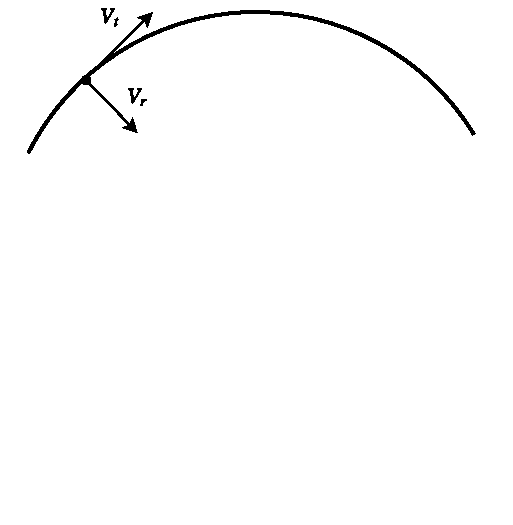
\includegraphics[width=\textwidth]{Vectors.pdf}
        \caption{Object Velocity Vectors}
        \label{fig:ObjectVelocityVectors}    
    \end{figure}
\end{center}

The objects orbiting within these ranges have corresponding periods (amount of time it takes for an object to orbit around the Earth once), this means that an object in the lower orbit has a higher period than that of the higher orbits. The periods for the two limits of the LEO objects are also found in table~\ref{tab:ObjectParameters}.

Based on a number of physical limitations, the system implemented will only be capable of detecting the space debris once it appears within the field of view (FOV). The FOV is discussed in section~\ref{sec:FieldOfView}. Figure~\ref{fig:ObservableCharacteristics} illustrates the system and how its relation to the Earth. 
The inner circle represents the Earths surface and point P represents the position of the system on the Earths surface.  
The outer circule represents the path of an object orbiting the Earth.
The lenghts in this image are not to scale and do not represent the real situation, however, this is used for illustrative purposes.
It is highly important to determine the amount of time it takes from when the object first enters the systems FOV, until the point where it exits the systems point of view.
In this case it is assumed that the object travels directly over the boresite of the system and so it will take the maximum amount of time to travel over the field of fiew. In most cases, the objects do not travel directly over the FOV, and will therefore not be within the FOV for a reduced amount of time.
This illustrates the system in order to create a few starting assumptions/criteria for the system.
As can be seen in this image, the angle that is measured can be taken from two different reference points: the center of the Earth and the point P. Based on this, it can be seen that the angles that these two points create are different. This implies that if one were to calculate the maximum distance that an object can be detected (assuming a maximum FOV angle from point P), one cannot make use of the angle $\alpha$ and the distances of this arc as it would not represent the actual distances of the objects because the circle that the objects orbits around is different to the circle that is assumed the system makes use of.
Numbers $1$ and $3$ represent the points at which the object enters and leaves the FOV, and point $2$ represents the position of the systems zenith.

\begin{center}
    \begin{figure}
        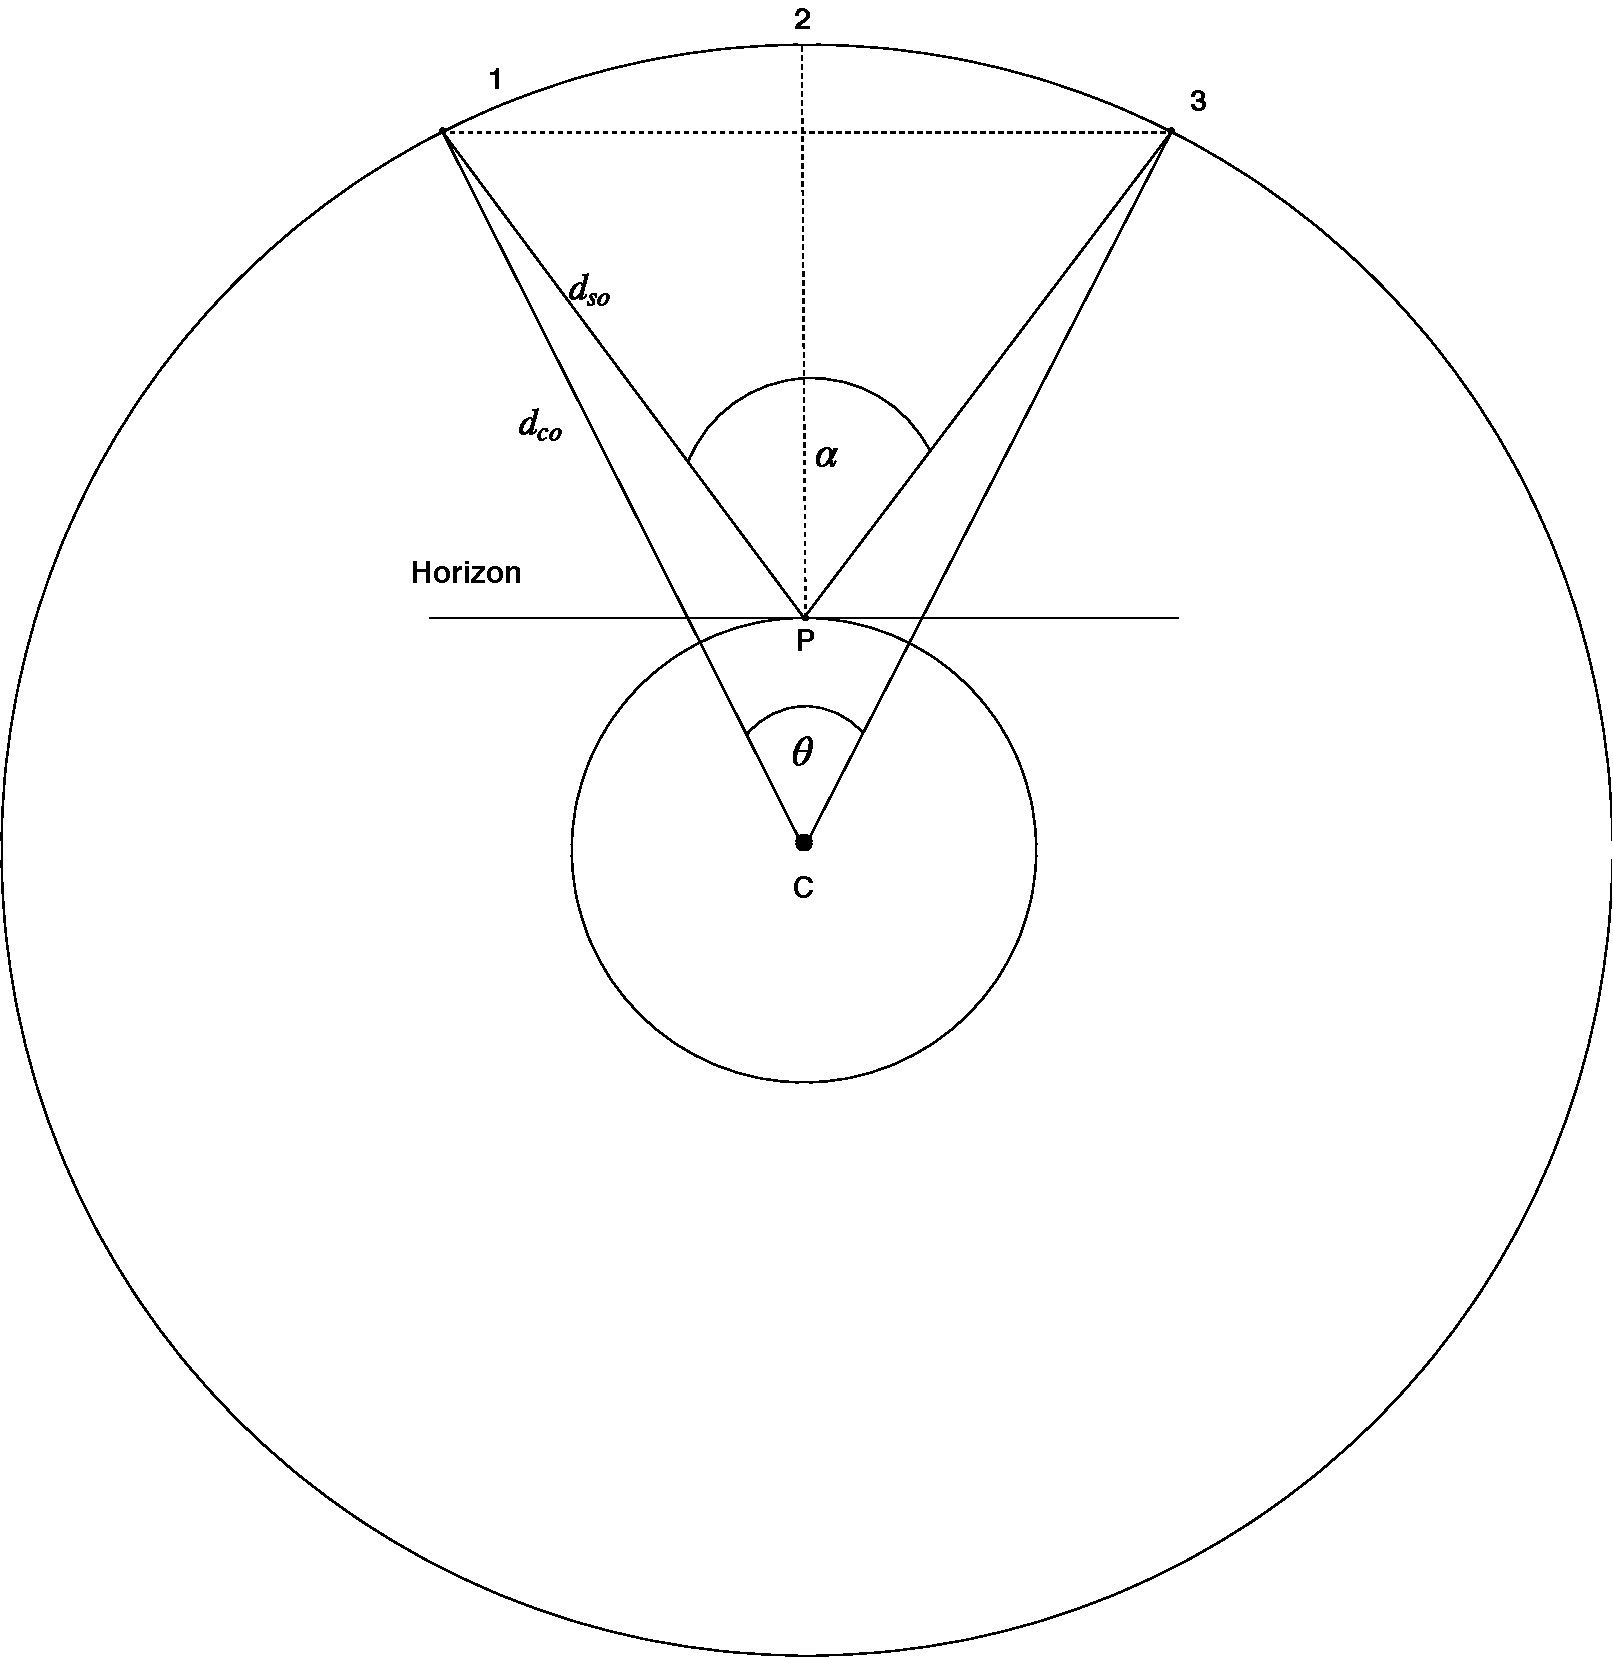
\includegraphics[width=\textwidth]{ObservableCharacteristics.pdf}
        \caption{Observable Characteristics}
        \label{fig:ObservableCharacteristics}    
    \end{figure}
\end{center}


Based on the movement of objects in differing orbits, it can be seen that objects in higher orbits move slower than those in lower orbits.
The objects move with a specific velocity, as illustrated in table~\ref{tab:ObjectParameters}, this is measured in linear velocity, however, it is also important to represent the motion of these objects with the use of their angular velocity, the angular velocity is simply found with the use of equation~\ref{eqn:AngularVelocity}.

\begin{equation} \label{eqn:AngularVelocity}
\omega = \frac{v}{r}
\end{equation}
Where:
\begin{itemize}
    \item $\omega$ represents the angular velocity of the object (Radians per second)
    \item $v$ represents the linear velocity of the object
    \item $r$ represents the distance from the observer to the object
\end{itemize}


Once this has been estimated, it is important to evaluate the angle travelled by the object as seen from the observation point ($\alpha_{p}$). This is measured over a period of time ($\Delta T$) and the angular velocity calculated above ($\omega_{P}$) is used, this is found in equation~\ref{eqn:AngularVelocityP}

\begin{equation} \label{eqn:AngularVelocityP}
    \omega_{P} = \frac{\theta_{P}}{\Delta T}
\end{equation}
Where:
\begin{itemize}
    \item $\omega_{P}$ is the same as before
    \item $\theta_{P}$ represents the angle of the object seen from the observation point
    \item $\Delta T$ represents the amount of time that it takes the object to traverse the angle
\end{itemize}

This now allows for the calculation of the linear velocity of the object as seen from the observation point (it is the same if the center of the Earth is used as the reference point). This velocity is calculated with the use of equation~\ref{eqn:LinearVelocity}.

\begin{equation} \label{eqn:LinearVelocity}
    v = \omega_{P} h
\end{equation}
Where:
\begin{itemize}
    \item $v$ is the linear velocity of the object (m/s)
    \item $\omega_{P}$ represents the apparent angular velocity of the satellite (Radians)
    \item $h$ represents the altitude of the object
\end{itemize}


The use of the two equations above require the values for the amount of time that it takes for an object to enter the FOV of the system and exit it again. This is found with the use of equation~\ref{eqn:ObservableTime} \cite{ObservableTime}.

% \begin{equation} \label{eqn:ObservableTime}
%     v = \omega_{P} h
% \end{equation}
% Where:
% \begin{itemize}
%     \item $v$ is the linear velocity of the object (m/s)
%     \item $\omega_{P}$ represents the apparent angular velocity of the satellite (Radians)
%     \item $h$ represents the altitude of the object
% \end{itemize}

% \begin{table}
%     \label{tab:ObjectParameters}
%     \caption{Orbject Parameters}
%     \begin{center}
%         \begin{tabular}[cc]
%             \hline \\
%             Minimum Object Altitude & $m$ \\
%             Maximum Object Altitude & $m$ \\
%             Maximum Object Tangential Velocity & $m/s$ \\
%             Minimum Object Tangential Velocity & b
%             Maximum Angular Velocity & \\
%             Minimum Angular Velocity & \\
%         \end{tabular}
%     \end{center}
% \end{table}

% What is an Antenna?
% What is an array?
% What is an antenna array?
% What is space?
% What is space debris? (How did it get there? why is it there? what is it made up of? where is it in space? how is it moving in space? is it bad/good? can we remove it? should we remove it, why? why do we care? who wants to know? fastest moving debris? how often do they come into contact with each other ? what happens when they come into contact with each other? can we protect against it? how is it currently being tracked?  )
% What are orbits?
% What is lower earth orbit? Geostationary orbit?
%  What is the atmosphere? (Range? made up of?)
%  What is the ionosphere? (Range? made up of? characteristics? EM characteristics? How fast can things move through them? )
%  current technology? radar and telescopes? advantages and disadvantages of these technologies?

The nature of an Incoherent Scatter Radar system is such that it directs electromagnetic energy into the earths "surrounding area"(ionosphere?); it highlights irregular characteristics present in this space. The energy that is transmitted is then reflected off of these irregularities and returns back in the direction of the system.
The system has the ability to create a narrow beam which transmits energy, this energy is then sterred (electronically) within the bounds of the system. Steering can be done in azimuth, elevation, and intensity. 
\section{CHOICE OF TECHNOLOGY}

\section{INDIVIDUAL AND ARRAY SIMULATIONS}


\subsection{Field of View} \label{sec:FieldOfView}

\section{COST OPTIMISATION}

\section{CHOICE OF PHYSICAL LOCATION IN SOUTH AFRICA}

\section{WHAT IMPACT WILL THE SYSTEM HAVE ON THE ENVIRONMENT}

\section{SENSITIVITY ANALYSIS}

\section*{ACKNOWLEDGEMENT} \label{sec:ACKNOWLEDGEMENT}


%%%%%%%%%%%%%%%%%%%%%%%%%%%%%%%%%%%%%%%%%%%%%%%%%%%%%%%%%%%%%%%%%%%%%%%%%%%%%%%
%
%\nocite{*}
\bibliographystyle{witseie}
\bibliography{references}


%{\tiny \vfill \hfill \today \hspace{5mm} witseie-paper-2003.\TeX}

\end{document}

" vim: ts=4
" vim: tw=78
" vim: autoindent
" vim: shiftwidth=4
